% 2 til 4 situasjonsfortellinger Teori og begreper flettes inn underveis Refleksjoner rundt situasjonene, både individ- og gruppenivå Aksjoner (tiltak/videreføre, reflektere)

\section{Kommunikasjonsmønster} %gruppelogg 08.02 
Under en av gruppens diskusjoner 8. februar fikk vi en tilbakemelding av fasilitator på hvordan kommunikasjonen i gruppen utartet seg. For å gå inn i dybden på dette kan det nevnes hvordan stemningen på gruppen var på starten av dagen. Onsdagen før fikk vi utviklet en idé som alle på gruppen var fornøyde med. Etter flere timers arbeid med dette hadde vi en oppsummering sammen med landsbyens leder for å oppdatere henne på hvordan vi lå an. Det viste seg at slik spillet var på dette stadiet var resirkulering ikke et stort nok fokus i spillet. Vi måtte derfor gjøre store konseptuelle endringer for å bedre kunne treffe landsbyens tema. Dette ble en dårlig avslutning på dagen, og motivasjonen sank betraktelig.

	\subsection{Demotivasjon til motivasjon}
	Da vi møtte opp onsdag 8. februar var den generelle stemningen på gruppen at medlemmene var demotiverte. Det at ideen vår fra den foregående onsdagen føltes som bortkastet lå fortsatt i tankene til alle på gruppen. Kjetil nevnte at han var lite klar for å gå tilbake til start og gjennom nye idémyldringer, ettersom vi forrige gang endelig følte at vi hadde en idé som alle var fornøyde med. Dette utsagnet var ikke akkurat noe som bidro til en bedre start på dagen for resten av gruppen. Trond og Andreas tenkte at man bare må gjøre det beste ut av det, og de startet en diskusjon som gikk ut på å dekomponere ideen vår fra forrige gang. Kjetil kastet seg på, og motivasjonen hans økte når han innså at dette kanskje ikke var verdens undergang. Etter en periode med ny brainstorming videreutviklet og endret vi det vi jobbet med forrige onsdag. Lydnivået økte og motivasjonen på gruppen steg blant flere av medlemmene. En ny idé ble født.

	\subsection{Individuelle oppfatninger}
	Da Andreas følte at gruppen virkelig var i sving, kom fasilitator bort til gruppen med en skisse som viste hvordan kommunikasjonen på gruppen var.

			\begin{figure} [here]
				\begin{center}
					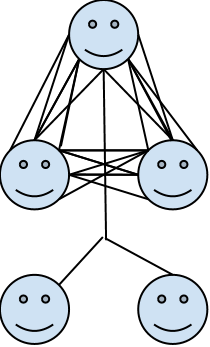
\includegraphics[scale=0.5]{communication}
				\end{center}
			\caption{Kommunikasjonsmønster}
		\end{figure}
		
%h	Place the float here, i.e., at the same point it occurs in the source text.
%t	Position at the top of the page.
%b	Position at the bottom of the page.
%p	Put on a special page for floats only.
%!	Override internal parameters LaTeX uses for determining `good' float positions.

	Dette kom som en overaskelse på gruppen. Det viste seg at Andreas, Kjetil og Trond var mest aktive, mens Ina og Christian var mer passive. Dette måtte diskuteres i gruppen.

	Ina mener at årsaken til hennes passivitet er i tråd med hennes vanlige oppførsel under et gruppearbeid. Hun legger til at hun er meget observant og enig i det som skjer, men at hun ikke alltid legger merke til at hun kan virke passiv for resten av gruppen. Når hun er enig tenker hun ikke over å si dette til resten av gruppen, eller gi de andre hennes godkjennelse. Hvis hun derimot er uenig sier hun ifra. Hun understreker at hun ikke er tilbakeholden eller ukomfortabel med å si ting foran hele gruppen. Ina sier at hun føler seg like aktiv som de andre selv om hun snakker mye mindre. Dette er derimot ikke resten av gruppens oppfatning, som i dette tilfelle oppfattet henne som passiv. Christian var veldig trøtt på morgenen, og merket at han var "litt i kjelleren". Etter en kaffekopp ble han dog mer deltakende i diskusjonen.

	Kjetil mener at det er lett at man uten å tenke over det henvender seg til de som er mest aktive, ettersom man får mer respons fra dem. Andreas sier at grunnen til at vi ikke inkluderer alle ikke har noe med at man trenger aksept fra enkelte av gruppenes medlemmer, men at diskusjonen hoper seg opp der folk er mest aktive. Dette observerte Andreas senere på dagen, da mønsteret flyttet på seg.
	% Den siste setninga må enten utdypes mer eller sløyfes-

	Etter at vi ble observante på hvordan dette mønsteret var, tok vi en pause; for å tenke litt på andre ting, ta en kaffe, og reflektere litt over hvorfor det var slik. Det var ingen tvil om at aktiviteten på gruppen ble mer balansert etter denne pausen. Vi ble klar over hvem vi henvender oss til når vi snakker. Andreas sa senere at han begynte å ta dette i betrakning i senere diskusjoner, der han beveger blikket mer for å få visuell kontakt med alle på gruppen. Trond foreslo at man kan legge til spørsmål til gruppemedlemmene om de er enige eller uenige, og rette disse mot dem på gruppen som er mer passive. Ifølge Schwarz \cite{Schwarz} er det å invitere til drøfting av egne innspill en god måte å øke effektiviteten i gruppen på. Dette bidrar til å få mer kommunikasjon mellom alle på gruppen, og inkludere dem som kan være umotiverte og trøtte eller ikke kommuniserer like mye. 

	% \subsection{Tittel} ?
	Gruppen ble også bevisst på et annet problem under videre diskusjon om spillideen – selv om ideen utviklet seg raskt og det var stor enighet i gruppen, så vi allikevel at når vi satte oss ned og tegnet ut ideene på hvert vårt papir at flere av oss så for oss ganske forskjellige ting. Selv om kommunikasjonen så ut til å fungere etter situasjonen om gruppens kommunikasjonsmønster, var det likevel store forskjeller i hva de forskjellige medlemmene trodde vi diskuterte. Her har Schwarz en teori om at man ved å dele all relevant informasjon, og alltid spille med åpne kort og konsekent avdekke resonnementene bak de innspillene man kommer med, vil man bedre kunne hjelpe gruppen i å arbeide effektivt sammen. Ved å gå mer i dybden på det vi diskuterer, snakke om detaljer og å være klar over at vi tenker forskjellig fører videre til at slike misforståelser blir unngått. Det å kartlegge slike ulikheter kan også brukes som en fordel i gruppen. I neste avsnitt reflekteres det over denne situasjonen i forhold til gruppemedlemmenes ulike tankegang.

	\subsection{Refleksjon} %johnson, kap 10
	Johnson og Johnson \cite{Johnson} understreker i sin artikkel viktigheten av mangfold i en gruppe, at ulike personligheter er en forutsetning for at gruppen skal være velfungerende. Det at gruppens medlemmer tenker forskjellig kan virke frusterende når man skaper en idé, men dersom gruppen klarer å kartlegge disse ulikhetene kan gruppemedlemmenes ulike tankegang bidra til å skape noe større og bredere enn hvis alle på gruppen hadde hatt helt lik tankegang. I vårt tilfelle er de personlige karaktererforskjellene blant annet kjønn, studieretning og ulike verdier og meninger, i tillegg til ulik erfaring og kunnskap. De på gruppen som studerer eller har studert datarelaterte emner, det vil si Kjetil, Trond og Christian, er noe mer likesinnede og har ofte like forestillinger under idéutviklingen. De tar hensyn til programmering og gjennomføring av spillet, noe som Andreas og Ina ikke tenker på, ettersom de ikke har noe kunnskap innen dette feltet. Ina og Andreas tar derimot andre ting i betrakning under idéutviklingen, hvor blant annet inkorporering av biologi og geologi i spillet står sentralt.

	% Flytte den litt ned, eller i allefall et annet sted.
	% Teori - erfaringer - forsettelse på den samme teorien blir litt rotete.
	Dette fører til at når vi i situasjoner kommer frem til noe alle er enige i, betyr ikke dette at man alltid vet \emph{hva man er enige om}. Fordi gruppens medlemmer, på grunn av deres ulike erfaringer og (ubevisste) preferanser, har ulike bilder i tankene om hvordan de ser for seg denne ideen. Vi fant ut at dette var tilfelle. Så hvordan kan vi dra nytte av dette?

	I utgangspunktet skulle man tro at en homogen gruppe som består av datastudenter er det optimale i gjennomførelsen av et slikt prosjekt. Johnson og Johnson nevner flere ulemper ved en lik gruppe. I denne situasjonen skal vi nevne en av disse ulempene. En slik gruppe kan mangle et bredt perspektiv. Kjetil, Trond og Christian ville antageligvis klart å lage et godt produkt, men med en homogen tankegang er det antageligvis mange ting de ikke ville ha tenkt på. Ina og Andreas, som ikke har kunnskaper innen programmering, ser på oppgaven i et annet perspektiv enn resten av gruppen. Selv om de har ikke noe å bidra med rent teknisk til resultatet, ser på ting annerledes og kaster lys over oppgaven på en måte datastudentene ikke tar i betrakning. Da vi prøvde å flette sammen hver persons synspunkt på hva vi trodde vi hadde kommet frem til, førte dette til at hele gruppen endret sin personlige idé over hva vi hadde diskutert og gjorde det om til gruppen sin idé. Dette resulterte i noe ingen på gruppen hadde sett for seg, men som alle var veldig fornøyde med.  Kjetil mente først at denne diskusjonen var sløsing og tid og så på dette som en unødvendig del av gruppearbeidet. Men den ideen gruppen satt igjen med på slutten av dagen fikk Kjetil til å tenke annerledes. Han ble overrasket over at hans eget syn på dataspillet vi utviklet ble såpass endret da de andre på gruppen fortalte hva de tenkte. 


	% Sette inn hvor det passer
Som datastudenter med programmeringserfaring er det alltid en overhengende fare for at en begrenser ideer ved å tenke at "dette er ikke mulig å gjennomføre", hvor en heller burde tenke "dette er vanskelig å gjennomføre", eller "dette kan ikke  \emph{jeg} gjennomføre". Det er det svært lurt å ikke legge for stor vekt på hva som er mulig og umulig. Det å involvere mennesker uten programmeringserfaring kan derfor være en fordel i slike prosjekter, spesielt, da det er slik i Eksperter i Team at et godt konsept stiller like sterkt som en god gjennomføring. 


Ulike synspunkt og meninger, i tillegg til ulik faglig kompetanse og tankegang, førte til et resultat ingen på gruppen så for seg i starten, men som alle var meget fornøyde med. Vi klarte med andre ord å dra nytte av synergieffektene som kommer av vår ulikheter.



\section{De Bonos hatter} %gruppelogg 14.03
14. mars hadde alle gruppene i landsbyen en midtveispresentasjon av prosjektet. Etter hver presentasjon skulle de andre gruppene ta på seg ulike roller ved bruk av metaforiske “hatter”, for så å evaluere presentasjonen og prosjektet til hver gruppe som fremførte. Denne tilbakemeldingsteknikken heter De Bonos hatter og er basert på Edward De Bonos' "Six Thinking Hats" \cite{bonos}

Prinsippet går ut på at menneskehjernen tenker på ulike måter som kan bli delt inn i forskjellige kategorier. Under denne øvelsen blir hver gruppe fortalt på forhånd hvilken kategori de tilhører, for dermed å gi tilbakmeldinger fra ulike synspunkt. Dette kan bli brukt som et verktøy for å skape en mer effektiv diskusjon, ettersom man systematisk får tilbakemeldinger fra hver kategori. Dette sikrer ulike relevante innfallsvinkler og hindrer fastlåsing.

Det er seks forskjellige kategorier man bevisst bruker i denne øvelsen, og hver av disse har fått tildelt en farget hatt som en metafor på de ulike tilstandene. De ulike kategoriene flettet inn i sitasjonen vår er:
\\
\\
\begin{tabular}{| l | l |}
\hline
\bf{Farge} & \bf{Tilstand} \\
\hline
Hvit hatt & Informasjon \\
Rød hatt & Følelse og intuisjon \\
Gul hatt & Muligheter \\
Svart hatt & Kritisk blikk \\
Blå hatt & Prosessblikk \\
\hline
\end{tabular}

\vspace{1.0em}

% \begin{description}
% \item[Hvit hatt - informasjon] \hfill \\
% Her skal man bruke fakta og informasjon og gi tilbakemeldinger fra et nøytralt og objektivt perspektiv. Den hvite hatten har som mål å finne ut hva man har av fakta og hvor man kan finne mer fakta. Det er viktig å ikke bruke følelser og egne meninger når man har denne oppgaven.

% \item[Rød hatt - følelse og intuisjon]\hfill \\
% Den røde hatten representerer egne følelser, både positive og negative. Man trenger ingen begrunnelse for hva man sier. Det er intuisjonen som er sentral.

% \item[Gul hatt - muligheter] \hfill \\
% Den gule hatten skal få frem positive sider og muligheter. Tilbakemeldingene skal være åpne og tankene skal være visjonære.

% \item[Svart hatt - kritisk blikk] \hfill \\
% Her har man rollen som dvelens advokat. Man skal identifisere negative sider, risokoelementer og svakheter. Samtidig er det viktig å være saklig og ha fokus på forsiktighet og sårbarhet.

% \item[Grønn hatt - kreativitet] \hfill \\
% Når man har på seg den grønne hatten er det ikke tillatt å gi kritikk. Man skal tenke kreativt og tenke over nye ideer og vekst for idèen man kommenterer.

% \item[Blå hatt - prosessblikk] \hfill \\
% Her må man tenke prosesstyring. Man skal kartlegge hvor langt gruppen har kommet i prosessen, hva som trengs å gjøre og hvordan man kan ta beslutninger for å komme i mål. \\
% \end{description}

		\begin{figure} [here]
				\begin{center}
					
\includegraphics[scale=0.5]{debonos}
				\end{center}
			\caption{De Bonos hatter}
		\end{figure}
		
		
Gruppen som hadde presentasjon fikk etter tur tilbakemeldinger fra de forskjellige hattene. Dette var en bra måte for å få startet en diskusjon. Det var også et verktøy som bidro til å hjelpe gruppen med sitt videre arbeid på prosjektet. Hver gruppe fikk prøve seg som hver hatt. Videre gjennomgår vi de ulike situasjonen vi var i som hver hatt, og hvordan det føltes og gå inn i de forskjellige rollene.

\subsection{De ulike rollene}
Under den første presentasjonsrunden ble vår gruppe tildelt den røde hatten (følelse og intuisjon). Vi var litt usikre på hvordan vi skulle håndtere dette, og hva vi skulle se etter under presentasjonen. Kjetil synes det ble litt rart å prøve å fokusere på spesifikke ting ved presentasjonen, men så i etterkant hvor nyttig dette var. Det var  kun Kjetil og Andreas som kom med uttalelser om sine følelser rundt presentasjonen. De andre på gruppen synes at det var vanskelig å fortelle hva en føler om en presentasjon. Men Andreas mente at man kun trengte å si det første man tenkte på, og at dette var en enkel oppgave. 

I den neste presentasjonsrunden ble vi tildelt den gule og hvite hatten. Disse var litt enklere å forholde seg til, ettersom vi skulle komme med positive tilbakemeldinger og være visjonære (gul hatt) og deretter spørre etter fakta og være nøytral (hvit hatt). Kjetil stilte spørsmål for å få frem mer informasjon, men følte egentlig ikke at han oppfylte rollen å ha som den hvite hatten.

Andreas syntes det var både positive og negative sider med den svarte hatten (kritisk blikk). Det var enkelt å gi konkrete tilbakemeldinger på hva som kunne forbedres eller hva man ikke likte, men Andreas syntes at det var litt ubehagelig og krevende å si noe kritisk og samtidig passe på at man ikke sier noe som sårer dem man snakker til.

Gruppen slet litt med å komme med innspill under den grønne hatten (kreativitet). Litt av grunnen til dette var at gruppen som presenterte allerede hadde en god idè, som var godt utviklet. Vi kom med noen innspill til dette, men Kjetil følte egentlig at vi var mer kritiske enn kreative, noe som gjorde rollen vanskelig.


\subsection{I sentrum av seks hatter}
Det å få vårt eget prosjekt tatt i fra hverandre på denne måten var en lærerik affære. Det ble pekt på en del elementer som vi selv har diskutert mye tidligere, spesielt valget mellom det å implementere spillet som sanntid eller turbasert. Av de tilbakemeldinger vi fikk kunne det virke som om andre så for seg at spillet ville fungere bedre som et turbasert spill. Det var og spørsmål om spillets moral, og om spillet vårt egentlig ville være lærerikt. Det virket dog som vi hadde tenkt på det meste som ble kommentert, og vi føler vi har god kontroll. Alt i alt følte vi dog at tilbakemeldingene vi fikk var av en positiv art, noe vi følte oss svært fornøyde med. Vi var spesielt fornøyde med tilbakemeldinger fra den røde hatten. Det gikk igjen at intuisjonen til de andre i landsbyen var at vårt konsept virket spennende og at man ikke burde utvide det noe videre. Den grønne (kreativitet) og gule (muligheter) hatten kom med flere interesante innspill. Men ingen av tilbakemeldingene her var ting vi ikke hadde diskutert tidligere i prosessen. De kritiske tilbakemeldingene vi fikk fra den svarte hatten og spørsmål knyttet til prosessen fra den blå hatten handlet i større grad om hvordan vi skal klare å publisere ideen vår og konkurrere mot tilsvarende spill. Christian mente at dette egentlig var positive kommentarer, ettersom det viste at de andre i landsbyen hadde stor tro på idèen vår. 


\subsection{Hvilke hatter har vi i gruppen?}
Det å ha rollen som den kritiske svarte hatten synes Andreas passet bra til ham, ettersom han ofte leter etter ting å være kritiske til i slike situasjoner. Utfordringen ligger i å velge ord med omhu. Han følte seg mest komfortabel med den røde hatten; å si hva han føler og mener uten begrunnelse. Dette passer bra med gruppens beskrivelse av Andreas. Andreas oppdaget også at enkelte av landsbyens medlemmer passet godt til den grønne hatten, ettersom det stadig var de samme deltakerne som kom med kreative innslag.

Christian syntes også at den svarte hatten passet bra til han. Han liker å være kritisk til nye idèer for å være en deltaker i forbedringer rundt dette. Dette passer bra til resultatet Christian fikk etter SPGR-øvelsen (se avsnitt 4?: Person gruppe relasjon), der han i den situasjonen så seg selv som en analytisk og påståelig person. Christian likte ikke den blå hatten. Han synes det var kjedelig å sette seg inn i en saklig og prosessrelatert rolle som ikke kom med egne meninger og innspill.

Trond syntes det var vanskelig å snevre inn sine tilbakemeldinger til en kategori. Han skulle ønske at man kunne være kritisk samtidig som man diskuterer muligheter og er kreativ. 

Kjetil likte best den rød hatten; å fortelle magefølelsen sin uten begrunnelse. Kjetil likte derimot ikke å ta på seg den kritiske rollen som en svart hatt, blandt annet fordi han selv måtte være observant på å identifisere negative sider ved presentasjonene. Han likte heller ikke at folk visste at han "nå skal den svarte hatten snakke", ettersom tilskuerne da forventer at han skal si noe negativt. De Bono beskriver dette som et av poengene med å metaforisk ha på seg en hatt. De andre skal vite hvilken rolle du har slik at du får oppmerksomheten rundt hvilken hatt du har på det. 

Ina deltok ikke på denne øvelsen, men har likevel prøvd å idenfisere seg selv som en av hattene. Hun stod mellom den hvite hatten og den gule hatten. Hun liker å ha en nøytralt syn og å fokusere på fakta og informasjon, samt snakke om muligheter og gi positive tilbakemeldinger. Hun liker ikke å være kritisk eller snakke om negative følelser, ettersom hun er redd for hva folk tenker om henne i slike situasjoner. De Bono legger vekt på at hattene vi metaforisk tar på oss er et kostyme som sjuler våre personligheter og kler oss ut som en bestemt person. Dermed kan man oppføre seg som den personen man har "kledd seg ut" som. Med dette i tankene mener Ina at hun kunne tatt på seg rollen som hvilken som helst hatt, men hun foretrekker den hvite og gule, ettersom dette reflekterer henne bedre i en dagligdags situasjon til vanlig.

Selv om vi ikke bruker denne øvelsen i gruppen, kan man se ut i fra hva gruppemedlemmene likte og ikke likte, hvilket personligheter som framkommer under en tilbakemeldingssituasjon eller diskusjon i gruppen. Gruppen er godt representert med deltakere som liker å være kritiske og fortelle om sine intuisjoner og følelser. Christian, Andreas og Kjetil faller i disse to kategoriene, som røde og svarte hatter. Trond er et godt kreativt samt kritisk bidrag, mens Ina liker best å snakke om informasjon og muligheter. Med dette er alle hattene, unntagen den blå, representert i gruppen. Dette er med til å bidra til en effektiv gruppe som får belyst idèer, muligheter og meninger fra forskjellig vinkler. 

Den blå hatten (prosessblikk) var det ingen på gruppen som kjente seg igjen i. Vi tenker at en slik person er en slags gruppeleder som har kontroll på hvordan gruppen ligger an, hva som må gjøres og hvordan man skal planlegge fremover. Kjetil mener at flere på gruppen egentlig har et prosessblikk på gruppearbeider, og at dette kanskje er noe man ikke tenker over. I tillegg har vi landsbylederen og fascilitatorene som følger oss opp. Dermed er alle hattene representert i gruppen vår.


Alle gruppemedlemmene syntes at De Bonos hatter var et nyttig verktøy. Det kan være en fin øvelse å bruke i utviklingsfasen av konseptet vårt. Vi bestemte oss for å ta en gjennomgang av hele prosjektet vårt en måned frem i tid ved bruk av De Bonos hatter. Dermed sikrer vi oss at alle aspekter blir tatt opp, og om det er noe vi kan endre/forbedre før vi sier oss fornøyde. Det er også viktig at alle på gruppen får være de forskjellige hattene, til og med de rollene man ikke liker. Det er for eksempel viktig at Ina og Kjetil tar på seg rollen som den kritiske. De andre på gruppen er ofte kritiske, men Ina og Kjetil sitter kanskje inne med kritikk de ikke vil ta opp som kan være avgjørende for prosjektets ferdigstilling. 



\section{Person- Gruppe Relasjon} %SPGR-øvelsen 21.03
Den 21. mars bestemte gruppen seg for å gjennomføre en SPGR- test (Systematisere Person-Gruppe Relasjonen). Det var tidlig på morgenen, og gruppemedlemmene hadde nettopp fått en kopp kaffe. Produktiviteten var lav, og muligheten til å kvikne til med en gruppeøvelse var forlokkende. Hensikten med denne øvelsen var å se på hvilke typer adferd som fant sted i gruppen, gitt en bestemt situasjon. 

Gruppen ble gitt 3 minutter til å bestemme seg for en situasjon de ville analysere. Generelt har det ikke vært noen store konflikter innad i gruppen, men det var to situasjoner som pekte seg ut som mer konfliktfulle enn andre. Den første situasjonen var valg av konsept, mens den andre situasjonen var en beslutning på om det endelige konseptet skulle spilles i sanntid eller om det skulle være turbasert. Den sistnevnte situasjonen ble valgt, da det var enighet om at det var gruppens mest konfliktfylte situasjon. Trond ønsket at spillet skulle være turbasert, mens de andre gruppemedlemmene så for seg at spillet skulle spilles i sanntid. Andreas var redd for at dette var et dårlig valg av situasjon, ettersom Trond stod alene mot resten av gruppen. Men Trond syntes det var ok. Resultatet kunne bli interessant.

Etter at en situasjon var valgt, ble hver enkelt deltaker gitt 5 minutter til å kartlegge sin egen adferd i den gitte situasjonen, etterfulgt av 10 minutter til å identifisere de andre gruppemedlemenes adferd. Endre Sjøvolds SPGR- figur ble brukt til å kartlegge hver enkelts adferd. Videre ble det gjennomført en felles gjennomgang på 25 minutter, hvor hver enkelt deltaker delte hvordan en så på sin egen adferd, etterfulgt av hvordan hver av de andre medlemmene hadde oppfattet denne personens adferd. 

-------------- Legg inn bilde av SPGR- figuren--------------

Her er en oversikt over resultatene fra øvelsen:
\begin{description}
\item[Andreas] \hfill \\
Andreas følte selv at han var autoritær, påståelig og utadvent. Han var redd for at han kanskje ble oppfattet som for kontrollerende, men ble overrasket da det viste seg at gruppen så på ham som samarbeidsvillig, oppmuntrende og demokratisk. 

\item[Kjetil] \hfill \\
Kjetil så på seg selv som kritisk, åpen og sammarbeidsvillig. Han følte også at han ble litt likegyldig etter hvert som diskusjonen utartet seg, og at det viktigste var å komme videre med prosjektet. Gruppen så på Kjetil som medfølende, utadvent og ser alle som likeverdige. Andreas følte det var Kjetil som dro i gang diskusjonen, og han så på Kjetil som kritisk og autoritær.

\item[Trond] \hfill \\	
Trond hadde identifisert seg selv som åpen, demokratisk og rasjonell. Han følte også at han kunne være tilbakeholden og betvile sine egne evner. Resten av gruppen så på Trond som støttende, effektiv og vennlig. Da Trond var den eneste som argumenterte for at spillet skulle være turbasert, ble han også sett på som tøff og påståelig i denne situasjonen. 

\item[Christian] \hfill \\
Christian mente selv at han var konkurranseinnstilt, påståelig og analytisk. Kjetil var enig i at han var litt påståelig og til tider likegyldig, men den overordnede oppfatningen gruppen hadde av Christian var at han var demokratisk, støttende og tillitsfull. Andreas følte seg hørt når han fortalte noe til Christian.

\item[Ina] \hfill \\
Ina synes selv hun var samarbeidsvillig, påståelig og medfølende. Men følte også at hun var noe varsom og betvilte sine egne evner. Andreas var enig i at Ina var samarbeidsvillig og medfølende, mens Christian følte hun var forsiktig, men bestemt. Gruppen så på Ina som både åpen og demokratisk.  

\end{description}
Fra denne øvelsen kan man se at samtlige gruppemedlemmer føler seg mer ekstreme i væremåten sin enn hva som oppfattes av resten av gruppen. Et eksempel på dette var at de fleste hadde markert seg seg selv som påståelige, men av andre hadde blitt markert som mer forståelsesfulle, åpne og samarbeidsvillig. Andreas lurte litt på om det kunne ha noe med at man på grunn av at man var enige med hverandre ikke oppfattet andre som påståelige da det de sier reflekterer det en selv mener. 

Fremover er det derfor viktig å ha fokus på at man ikke blir for passiv. Fordi selv om man føler seg veldig dominerende, er det ikke sikkert at det er slik resten av gruppen oppfatter denne personen. Det er derfor ikke noe i veien for at gruppemedlemmene legger seg litt mer frampå og våger mer.


%Felles refleksjon om temaet, inkl:

%	* Ledelsesstruktur
%	* Polarisering (motsetningsforhold mellom ulike typer atferd)
%	* Behov som må oppfylles (manglende adferd)
%	* Ansvarsfordeling
%	* Forpliktelser
%	* Deling av informasjon
%	* Vanskelige eller ubehagelige tema
%	* Beslutningsprosesser
%	* Er de tre grunnleggende gruppefunksjonene til Sjøvold til stede? (Kontroll, Omsorg, og Opposisjon)
